\documentclass[twocolumn, linenumbers, superscriptaddress, nofootinbib]{revtex4-1}

\usepackage{amsmath}
\usepackage{graphicx}
\usepackage{gensymb}
\usepackage{textgreek}
\usepackage{xcolor}
\usepackage[colorlinks]{hyperref}
	\hypersetup{colorlinks,
	linkcolor={red!50!black},
	citecolor={blue!60!black},
	urlcolor={blue!40!black}
	}
\graphicspath{{figures/}}
%-------------------------------------------------------------------------------

\begin{document}
	\begin{abstract}
		The acorn weevil snout exhibits remarkable flexibility and toughness that are derived from from the microarchitecture of its exoskeleton.
		Here we characterize modifications to the composite profile of the rostral cuticle that simultaneously enhance the flexibility and fracture toughness of the distal portion of the snout.
		Using Classical Laminate Plate Theory (CLPT) we estimate the effect of these modifications on the elastic behavior of the exoskeleton.
		Additionally, changes in the relative layer thicknesses and orientation angles of layers in the exoskeleton are related to the tensile behavior of the snout in six species of diverse morphology, and we demonstrate that a highly curved rostrum can be completely straightened without structural damage.
		We demonstrate that increased endocuticle thickness is strongly correlated with increased tensile strength in the snout.
		Consequently, snout stiffness is shown to be inversely correlated with fracture toughness.
		Finally, we identify exocuticle rich invaginations of the occipital sutures both as a likely site of crack initiation in tensile failure and as a source of morphological constraint on the evolution of the snout.
		
	\end{abstract}
	
	%title and author block
	{\title{Exoskeletal strength and cuticle composite profile of the acorn weevil rostrum}
	\date{\today}
	
	\author{M. Andrew Jansen}
		\email[corresponding author, email:~]{majanse1@asu.edu}
		\affiliation{School of Life Sciences, Arizona State University, Tempe, AZ 85287, USA}
	\author{Jason Williams}
		\affiliation{School for Engineering of Matter, Energy, and Transport, Arizona State University, Tempe, AZ 85287, USA}
	\author{Nikhilesh Chawla}
		\affiliation{School for Engineering of Matter, Energy, and Transport, Arizona State University, Tempe, AZ 85287, USA}
	\author{Nico M. Franz}
		\affiliation{School of Life Sciences, Arizona State University, Tempe, AZ 85287, USA}
		
	\maketitle
	}

	The exoskeleton of Coleoptera (beetles) is a hierarchically-structured fibrous composite characterized by variously arranged \textalpha-chitin (N-acetylglucosamine) nanofibrils embedded in a heterogeneous protein matrix \cite{Hepburn1973, Jansen2016, Vincent2004}.
	Although \textalpha-chitin is brittle and strongly anisotropic, beetle cuticle is simultaneously rigid and tough due to its unique laminate microstructure (see kamp, vincent for review), which we characterize in detail below \cite{Kamp2010, Kamp2015, Neville1976}.
	Impact-prone areas and exaggerated structures in arthropods generally exhibit cuticle organization that resists deformation and fracture (e.g. \cite{Amini2015, Mccullough2014mech, Mccullough2014struc, Dirks2012, Dirks2013}); however, acorn weevils in the genus \textit{Curculio} Linnaeus, 1758\footnote{
		Pursuant to the International Code of Zoological Nomenclature, the first mention of any specific epithet will include the full genus and species names as a binomen (two part name) followed by the author and date of publication of the name.
		This is not an in-line reference; it is a part of the name itself and refers to a particular species-concept as indicated in the description of the species by that author \cite{ICZN1999}.}
	instead exhibit unusual distal flexibility in an elongate extension of the head called the rostrum (snout) \cite{Toju2005, Jansen2016, Singh2016, Gibson1969}.
	The rostrum is a hollow, strongly curved (over 90$\degree$ in some species), cylindrical, exoskeletal extension of the otherwise nearly-spherical head, which bears at its apex the terminal chewing mouthparts \cite{Morimoto2003, Ting1933, Ting1936, Dennell1942, Gibson1969}.
	This structure is used by the female to feed and to excavate sites for egg-laying (oviposition, see Fig.~\ref{fig::curculio}), and can be repeatedly bent without evident damage despite being composed of the same material as other rigid body parts \cite{Jansen2016, Singh2016, Gibson1969, Toju2005}.
	By maintaining constant pressure on the snout and rotating around the bore-hole, females are able to flex the rostrum into a straightened configuration and produce a linear channel into the fruit; a single female may prepare hundreds of such sites as an adult \cite{Toju2005, Moffett1989, AguirreUribe1978}.
	
	While this behavior has been observed in many species of \textit{Curculio} \cite{Gibson1969, Moffett1989, AguirreUribe1978, Toju2005}, it was unclear how the rostrum of female acorn weevils can withstand the repeated, often extreme bending incurred during the process of egg-chamber excavation.
	In this study we characterize the composite profile of the rostral cuticle to account for the observed flexibility of the snout.
	We show that the relative layer thicknesses and fiber orientation angles of the exocuticle and endocuticle of the rostrum are strongly differentiated from the head capsule and other body parts, and we estimate the effect of these differences on the elasticity of the cuticle using Classical Laminate Plate Theory (CLPT).
	Because recent studies have shown that the yield strength of the beetle exoskeleton is lower in tension than compression \cite{Longhai2017}, we perform a comparative analysis of the ultimate tensile strength of the rostrum across species and snout morphotypes; we also report the results of displacement-controlled load cycling of the snout in a species with strongly curved morphology.
	We relate an observed increase in the volume fraction of endocuticle in the rostrum to higher tensile strength at the rostral apex in all tested species, and find that a strongly curved rostrum can be flexed repeatedly without harm to the structure.
	
	\begin{figure*}
		\centering
		\includegraphics[width=180mm]{fig1.pdf}
		\caption{\textbf{Morphology and oviposition behavior of female \textit{Curculio}.} 
			\textbf{a}, Lateral habitus image of female \textit{Curculio~sayi} ((Gyllenhal, 1836)) featuring the elongate, strongly curved rostrum.
			\textbf{b}, Lateral view of the head of a female specimen of \textit{Curculio~longinasus}, with major anatomical features indicated.
			\textbf{c}, Illustration of the oviposition behavior of female \textit{Curculio}, proceeding from left to right: a female makes an incision in the host fruit, flexes the head directly over the bore hole using the front legs, then maintains tension on the snout while rotating to excavate a linear channel into the fruit. During this process, the rostrum is bent until completely straight.
		}
		\label{fig::curculio}
	\end{figure*}
	
	We additionally describe the fracture mechanics of the snout and consider how modification of the cuticle may prevent crack formation during oviposition.
	Based on our findings, we posit that the composite profile of the rostral apex enables the snout to undergo repeated distal flexion while remaining within the elastic limits of the material, mitigating the risk of structural damage, and without evident alteration of the mechanical properties of the individual components of the cuticle across the structure and between species.
	Thus, the flexibility and tensile strength of the rostrum appear to be derived \emph{exclusively} from modification of the composite architecture of the exoskeleton.
	To our knowledge, this is the first time that a modified composite profile has been reported as a means of enhancing structural elasticity in the insect exoskeleton (but see \cite{Matsumura2017}).
	
	\section{Microstructure of the \textit{Curculio} rostrum}
		In arthropods (including beetles), the exocuticle is comprised of numerous unidirectional laminae of chitin nanofibrils; each layer is the thickness of a single fiber (2-4\,nm) embedded in a proteinaceous matrix \cite{Nikolov2010, Nikolov2011}.
		These layers are stacked at a more or less constant angle to each other, forming a quasi-isotropic laminate known as the Bouligand structure \cite{Blackwell1980, Bouligand1972, Neville1976}. 
		This layout effectively mitigates the strong anisotropy of \textalpha-chitin to yield a versatile building material for the exoskeleton \cite{Vincent1982, Vincent2004, Nikolov2010, Nikolov2011}.		
		Beetle endocuticle, however, is unique among arthropods and is comprised of large (1-5\,{\textmu}m diameter in \textit{Curculio}) unidirectional bundles of chitin, called macrofibers.
		Chitin macrofibers are orthotropic (axial: $E_1~=~8.5\,\text{GPa}$, transverse: $ E_2~=~E_3~=~0.52\,\text{GPa}$ \cite{Jansen2016}) and arranged in unidirectional plies, seen in Figs.~\ref{fig::cuticle},~\ref{fig::profile} \cite{Kamp2010, Kamp2015}.
		Typically, adjacent macrofiber laminae are paired and pseudo-orthogonal (i.e., angled approx. $90\degree$ to each other \cite{Cheng2009}, see Fig.~\ref{fig::profile}), with a constant stacking angle \emph{between} pairs, although other configurations have been observed \cite{Hepburn1973, Kamp2010, Kamp2015, Leopold1992}.
		This geometric sequence of the macrofiber laminae yields an approximately transversely isotropic composite, similar to the Bouligand structure \cite{Kamp2015, Nikolov2010}.
		Notably, the resulting laminate is less rigid than the exocuticle, but exhibits greater toughness because the pseudo-orthogonal plies effectively inhibit crack formation and propagation between successive layers \cite{Kamp2010, Kamp2015, Hepburn1973}.
		
		\begin{figure*}
			\centering
			\includegraphics[width=180mm]{fig2.pdf}
			\caption{\textbf{Gross divisions of cuticle in the rostrum.}
				\textbf{a}, Scanning electron micrograph of the head capsule, in frontal view, of female \textit{Curculio~sulcatulus} (Casey, 1897), with the rostrum removed.
				\textbf{b}, Magnified view of the junction between the rostrum and head capsule showing the division of the cuticle into two general regions: the exocuticle and the endocuticle.
			}
			\label{fig::cuticle}
		\end{figure*}
		
		Serial thin sectioning and scanning electron microscopy of fractured \textit{Curculio} specimens revealed that endocuticle in the head capsule fits this general profile, with an angle of approximately $30\degree$ between successive pairs of pseudo-orthogonal plies.
		Additionally, in the head capsule, the thickness of the exocuticle and endocuticle in cross section are nearly equal (typically between 20-30\,{\textmu}m).
		However, we found that the cuticle composite lay-up of the rostral apex is strongly differentiated from the head capsule (Fig.~\ref{fig::profile}).
		Distally the exocuticle is reduced to a thin shell (ca. 5\,{\textmu}m), with the endocuticle thickened to offset this reduction and maintain a constant cuticle thickness (ca. 50\,{\textmu}m total) throughout its length.
		Moreover, the endocuticular macrofibers exhibit no rotation between successive pseudo-orthogonal plies, and are oriented at approximately $\pm45\degree$ to the longitudinal axis of the snout (i.e., an antisymmetric $[\pm45\degree]$ angle-ply laminate).
		We previously identified these modifications to the composite structure of the cuticle within a single species, \textit{C.~longinasus} Chittenden, 1927 \cite{Jansen2016, Singh2016}; however this composite profile has now been uncovered in the rostrum of six additional, phylogenetically disparate, species (detailed in methods), indicating that this is likely a genus-wide trait.
		In all examined species, the portion of the snout between the head capsule and apex of the scrobe exhibits a gradual transition in composite profile along an anterior-posterior gradient.
		
		\begin{figure*}
			\centering
			\includegraphics[width=180mm]{fig3.pdf}
			\caption{\textbf{Composite profiles of rostral cuticle.}
				\textbf{a}, Scanning electron micrograph of a fractured specimen of \textit{Curculio~humeralis} (Casey, 1897), showing that the cuticle of the rostral apex is organized as a $\pm45\degree$ angle-ply laminate..
				\textbf{b}, Scanning electron micrograph of a fractured specimen of \textit{Curculio~caryae}  (Horn, 1873), showing that the cuticle of the rostral base and head capsule has a roughly $30\degree$ stacking angle between each pair of pseudo-orthogonal plies.
				Semi-thin sections of cuticle from a specimen of \textit{C.~humeralis}, stained with toluidine-blue-borax, demonstrating:
				(\textbf{c}) that the exocuticle of the rostral apex is reduced to a thin shell close to 5\,{\textmu}m thick, with the endocuticle thickened to maintain a constant laminate thickness; and,
				(\textbf{d}) that the exocuticle of the head capsule and base of the snout occupies nearly half of the through-thickness of the cuticle.
			}
			\label{fig::profile}
		\end{figure*}
		
		We estimated the effect of differential cuticle organization on uni-axial membrane and transverse-flexural Young's moduli of the cuticle in the rostral apex and head capsule using Classical Laminate Plate Theory (CLPT), as detailed in our methods \cite{Reddy2004, Jones2014}.
		The effective elastic constants of the cuticle regions of \textit{C.~longinasus} (estimated previously, see \cite{Jansen2016}) were used to construct constitutive equations for the entire cuticle of that species.
		The cuticle of the head capsule was estimated to have membrane and flexural moduli of $E_m~=~4.77\,\text{GPa}$ and $E_f~=~6.04\,\text{GPa}$, respectively; however, in the rostral apex we found that these values were reduced by approximately 72\% and 60\%, respectively ($E_m~=~1.36\,\text{GPa}, E_f~=~2.44\,\text{GPa}$).
		Two hypothetical cuticle lay-ups were also modeled to individually assess the contributions of either modified layer thickness or stacking angle sequence to cuticle flexibility.
		The effective moduli of a configuration with the angle stacking sequence of typical cuticle (i.e., in the head capsule) but possessing the layer thicknesses of the rostral apex were calculated as $E_m~=~3.73\,\text{GPa}, E_f~=~4.31\,\text{GPa}$, representing 22\% and 29\% decreases from unmodified cuticle, respectively.
		Similarly, a hypothetical cuticle with the layer thicknesses of ordinary cuticle but possessing the angle stacking sequence of the rostral apex (i.e., $\pm45\degree$ angle-ply in the endocuticle) had effective elastic moduli of $E_m~=~3.77\,\text{GPa}, E_f~=~5.76\,\text{GPa}$, representing 21\% and 4.7\% decreases from unmodified cuticle, respectively.
		Each of the cuticle modifications noted in the rostral apex individually decreased the elastic moduli of the cuticle; however, they appear to have a synergistic combined effect on cuticle elasticity, rather than a simple additive effect.
		This result suggests that both modifications are necessary in order for the snout to function properly in the living animal, where the combined effect allows the rostrum to bend until completely straight without fracture.
		
	\section{Force-controlled loading to fracture}
		
		\begin{figure*}
			\centering
			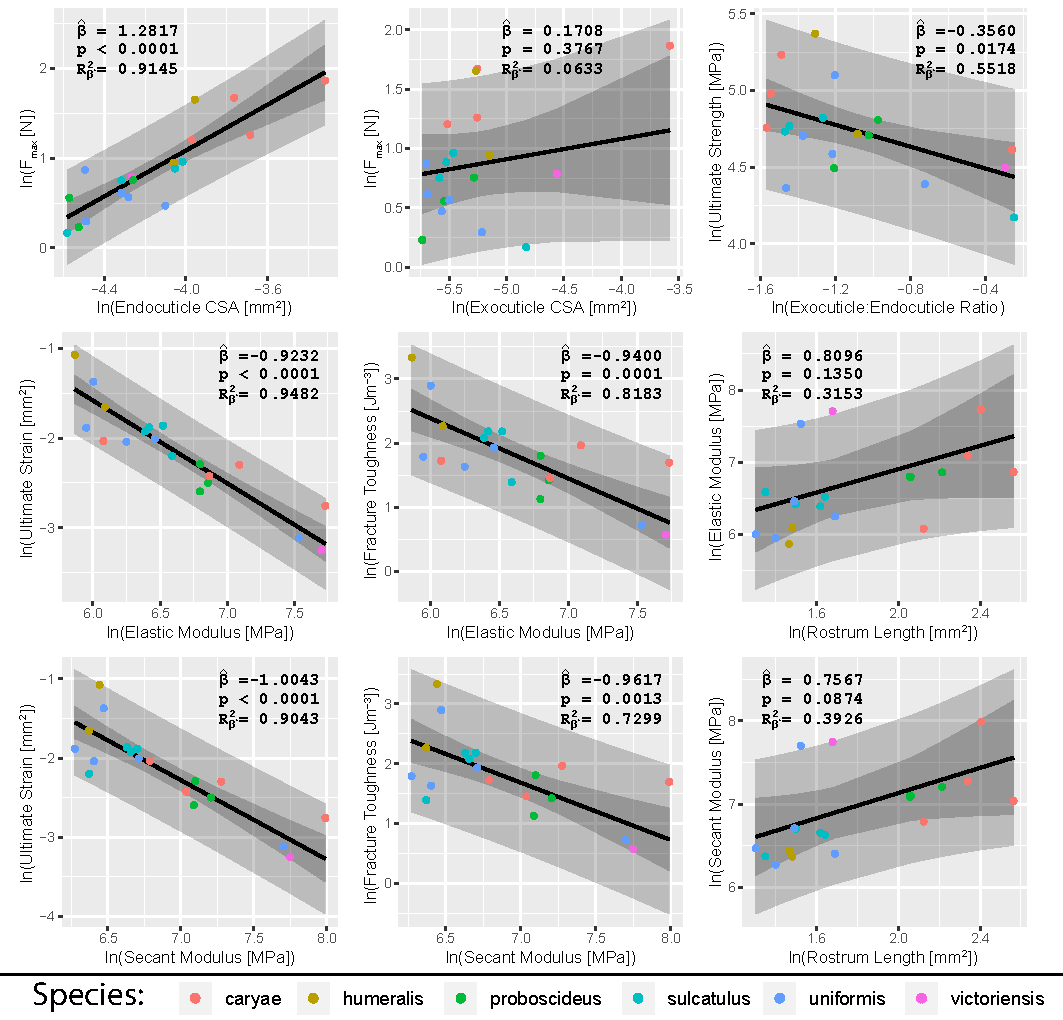
\includegraphics[width=180mm]{fig4.pdf}
			\caption{\textbf{Tensile properties of the \textit{Curculio} rostrum.}
				Each plot shows the relationship between two variables as predicted by a phylogenetic linear mixed-effect model, with species as a random effect and a variance-covariance matrix generated from Brownian motion over the preferred phylogeny of Bonal et al. \cite{Bonal2016}.
				The gray regions represent the prediction interval and bootstrapped 95\% confidence interval of the model.
				The estimated fixed effect $\hat{\beta}$ is given, along with the p-value of a t-test assessing whether $\hat{\beta}$ is significantly different from zero.
				Also reported is a generalized marginal $\text{R}^2_{\beta^*}$ for assessing fixed effects (see online Methods for more information).
				In general, we find that increased endocuticle thickness is associated with greater tensile strength, and that stiffness is inversely correlated with toughness.
			}
			\label{fig::tensile}
		\end{figure*}		
	
		To better characterize the failure behavior of the rostrum, we performed tensile testing on the snouts of six \textit{Curculio} species that representing a mixture of closely and distantly related taxa (see Methods) \cite{Hughes2004phylo, Hughes2004eco, Bonal2016, Bonal2011}.
		Each specimen was immersed in $\text{di-H}_2\text{O}$ for 24 hours, to simulate the living tissue (see \cite{Klocke2011}), then subjected to force-controlled, uniaxial loading to fracture at a constant stress rate of $1.0\,\text{gf}\cdot\text{s}^{-1}$ (detailed in Methods).
		In general, the specimens exhibited a non-linear viscoelastic response curve characterized by a sharp increase in stress at higher strains, terminating in brittle fracture \cite{Mihai2017}.
		We postulate that strain hardening occurs as the longitudinal axis of the macrofibers becomes more closely aligned to the cylindrical axis of the rostrum, thereby resisting tension more directly with increasing strain \cite{Munster2013}.
		
		We examined the correspondence between composite structure and mechanical behavior of the snout using phylogenetic linear mixed effects models (PGLM, Fig.~\ref{fig::tensile}) to account for phylogenetic non-independence in residual variance, with species membership included as a random effect \cite{Revell2010, Felsenstein1985}.
		Our models show that the maximum force sustained at the site of failure was strongly correlated with the cross-sectional area of the endocuticle ($\hat{\beta}=1.28, p<0.0001$), and not the exocuticle ($\hat{\beta}=0.17, p=0.38$), at that site.
		Accordingly, there was a negative correlation between ultimate tensile strength of the specimen and the ratio of exocuticle to endocuticle cross-sectional area at the site of fracture ($\hat{\beta}=-0.36, p=0.017$).
		Although CLPT predicts a positive association between the proportion of exocuticle and stiffness of a generalized cuticle, we found no evidence of correspondence between the cross-sectional properties of the fracture site and the gross behavior of the entire rostrum.
		Because the cross-sectional areas of the cuticle regions vary across the length of the head along an anterior-posterior gradient, it is not possible to correlate measurements from the fracture surface to the properties of the entire snout.
		
		Instead, we found that the uniaxial elastic modulus (low strain: $E_{low}$) and secant modulus at failure ($E_{sec}$) were inversely correlated with ultimate strain and fracture toughness (see Fig.~\ref{fig::tensile}), implying that stiffer specimens, and by extension, stiffer cuticle profiles, are generally more brittle.
		We also observed a moderate, but not statistically significant, stiffening size-effect with respect to rostral length, contrary to our expectation that a longer, more strongly curved (see \cite{Hughes2004eco, Bonal2011}) snout would require increased flexibility to avoid fracture during oviposition.
		One possible explanation for this trend might be that longer snouts have a longer transition gradient from basal to apical profile to reinforce the junction between the rostrum and head capsule against buckling.
		Thus, Young's modulus of the rostrum would be comparatively higher in these species because of the higher volume fraction of exocuticle.
		From these tests, we infer that the gross elastic behavior of the cuticle is consistent across the genus, and that a single mechanism (i.e. the modified composite profile) confers increased flexibility and tensile strength to the rostral apex in the genus \textit{Curculio}.
		In addition, the endocuticle demonstrably contributes more to rostral tensile strength than the exocuticle, likely because of its organization into large bundles of aligned, anisotropic fibers, leading to a trade-off between rigidity and toughness.
		Consequently, the altered composite profile of the cuticle in the rostral apex makes the rostrum simultaneously more flexible and fracture resistant.
		
	\section{Load cycling of \textit{Curculio caryae}}
		
		\begin{figure*}
			\centering
			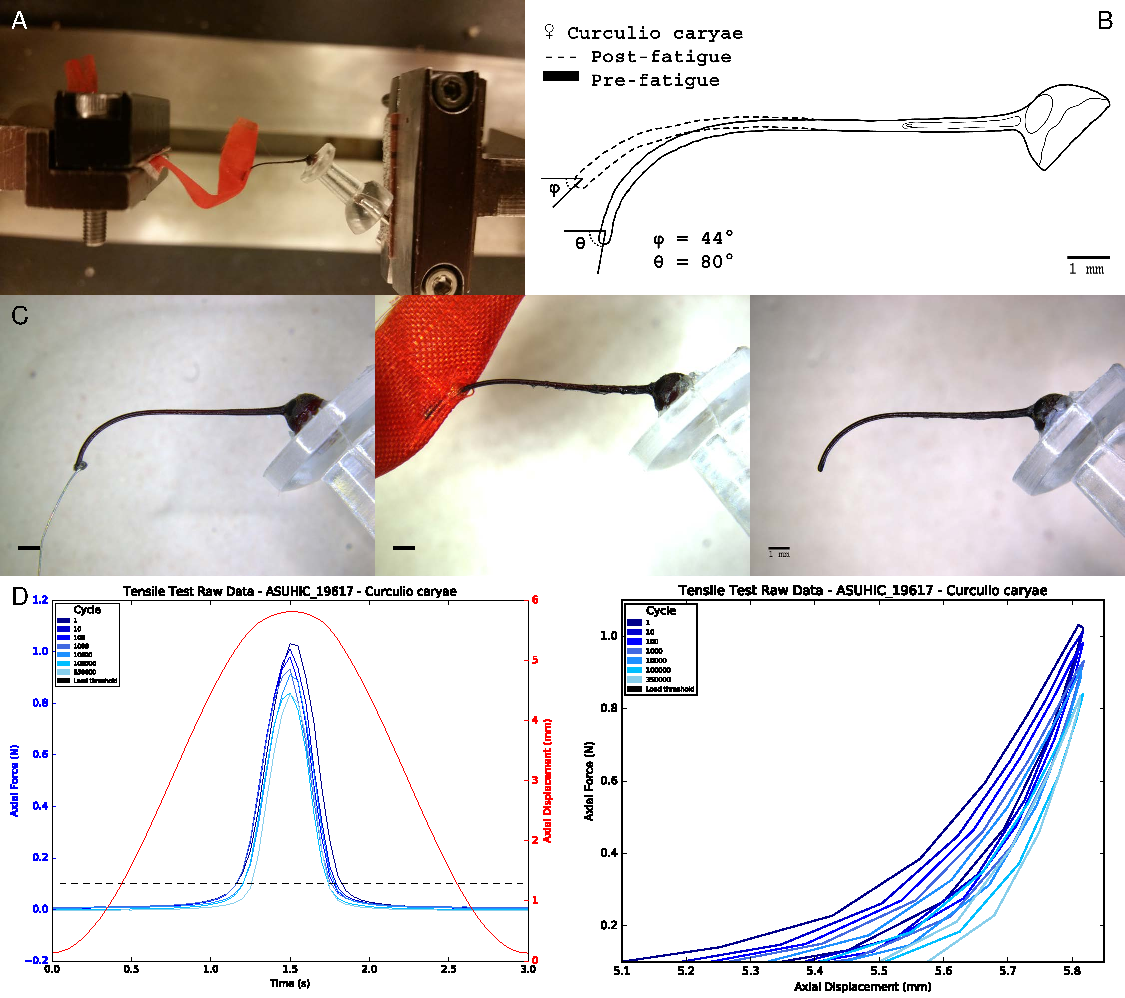
\includegraphics[width=180mm]{fig5.pdf}
			\caption{\textbf{Fatigue testing of a female C. caryae.}
				\textbf{a}, Shows the fatigue testing setup, wherein the head capsule was fixed to a pedestal and the rostrum was attached to a strip of rip-stop nylon fabric using cyanoacrylate adhesive.
				The specimen was loaded in tension, and not compression, isolating the effect of tension on the fatigue behavior of the rostrum.
				\textbf{b}, An overlay of the pre- and post-fatigue states of the head show a clear effect from repeated proscribed strain; however,
				\textbf{c}, Demonstrates that this effect is apparently not permanent.
			The first two panels to the left correspond to the pre- and post-fatigue states of the rostrum, respecively, but the third panel shows that the head has returned to its original shape after 24 hours soaking in a water/ethanol mixture.
				\textbf{d}, The two plots presented here are the raw force and displacment data from the fatigue test.
				The plot on the right shows clear viscoelastic behavior, indicated by histeresis in the stress-strain response of the specimen, and exhibits a logarithmic decrease stress amplitude over time.
			}
			\label{fig::fatigue}
		\end{figure*}
		
		To confirm that repeated, proscribed straightening of the rostrum does not result in damage to the cuticle, we performed displacement-controlled fatigue testing on a typical female specimen of \textit{Curculio caryae}, a species that exhibits extreme ($80-90\degree$, Fig.~\ref{fig::fatigue}) rostral curvature \cite{AguirreUribe1978, Gibson1969}.
		The specimen was aligned so that uniaxial tension would induce elongation of the distal portion of the rostrum with minimal off-axis deflection of the un-curved section.
		The strain per cycle was fixed at an amplitude sufficient to completely elongate the snout and generate a tensile load of 1.0\,N  in the straightened configuration (ca. 20\% ultimate strength) at a frequency of $0.33\,\text{Hz}$.
		The test was terminated after a period of two weeks (ca.~400K cycles) when the stress amplitude appeared to reach an asymptotic minimum.		
		The rostrum behaved viscoelastically, indicated by histeresis in the stress-strain relationship during each cycle.
		Strain amplitude decreased logarithmically with cycle number, and the specimen initially appeared to have deformed plastically during the test.
		We believed that this indicated damage to the specimen; however, after cleaning the specimen in a 24 hour wash with ethanol and water, we observed that rostrum returned to its original shape (Fig.~\ref{fig::fatigue}).
		
		We cannot fully account for the stress relaxation of the rostrum after testing, but we speculate that it arose from the general mechanism associated with cuticle viscoelasticity.
		The endocuticle is made of aligned \textalpha-chitin nanofibrils whose crystalline structure is enforced by hydrogen bonds between individual chitin chains and with the protein matrix along their length; macroscopic viscoelastic behavior results from slippage between these chains in response to shearing between the chitin molecules \cite{Vincent2004, Evans1967, Sun2012}.
		We posit that repeated strain may have caused such slippage in the endocuticle of the rostral apex during the fatigue test; however, without sufficient time for the material to \textit{completely} relax after deformation, the specimen would slowly accumulate strain and deform viscoelastically \cite{Munster2013}.
		After immersion in ethanol and water, the cuticle would be sufficiently plasticized to allow the specimen to return to its original configuration, dissipating the accumulated strain.
		
		The specimen did not show any evidence of fractures, micro-tears, or shear cusps anywhere in the surface of the exocuticle, and, furthermore, the tensile strength of the specimen was consistent with other members of its species ($F_max~=~5.02\,\text{N}$).
		Given this surprising result, it appears that the specimen was undamaged by the testing.
		We therefore expect that under normal conditions in life, repeated bending of the snout does not exceed the yield strength of the cuticle.
			
	\section{Fractography of test specimens}
		
		\begin{figure*}
			\centering
			\includegraphics[width=180mm]{fig6.pdf}
			\caption{\textbf{Fractography of the \textit{Curculio} rostrum.}
				\textbf{a}, Light micrograph showing the fracture surface of a tensile tested rostrum, in the species \textit{C.~caryae}, exhibiting a typical failure mode, illustrated in (\textbf{b}).
				The small, black arrows indicate the winding direction of the macrofiber lamina; green arrows and dotted lines indicate the direction of crack.
				Scanning electron micrographs highlight: (\textbf{c}) shear cusp formation, (\textbf{d}) tensile failure and off-axis macrofiber fiber-pulling, (\textbf{e}) interlaminar delamination, (\textbf{f},\textbf{h}), crack formation near invaginated exocuticle (\textbf{g}) ventral crack-front coalescence and shear cusp formation.
			}
			\label{fig::fracture}
		\end{figure*}
		
		Although it was not always possible to identify void nucleation and crack initiation sites given the complex failure modes evident in the fractured specimens, we observed several patterns characteristic of both the micro-scale behavior of the cuticle and the meso-scale behavior of the rostrum during uniaxial tensile failure (Fig.~\ref{fig::fracture}), which we describe here.
		
		In transverse view, the exocuticle consistently presented a nearly continuous fracture surface, characteristic of comparatively brittle failure, presumably due to the relatively homogeneous arrangement of \textalpha-chitin laminae in the Bouligand structure \cite{Nikolov2010, Nikolov2011}.
		The exocuticle typically appeared to fracture at lower strains than the endocuticle, with shear-cusp formation evident both at the fracture surface and across exocuticle adjacent to the plane of fracture \cite{Greenhalgh2009}.
		Conversely, the endocuticle exhibited severe delamination, off-axis ply-splitting, and fiber-pulling away from the fracture surface, indicating the relatively high toughness of the unidirectional \textalpha-chitin organization within the macrofibers \cite{Kamp2010, Kamp2015}.
		Because the exocuticle of weevils is anchored to the endocuticle by cross-linking fibers (see \cite{Kamp2015, Longhai2017}), exocuticular shear-cusp formation in uniaxial tension suggests extension-shear coupling within individual endocuticle laminae, implying that ply-splitting occurred via mode II fracture between macrofibers at high strain \cite{Jones2014, Reddy2004}.
		We hypothesize that intra-laminar extension-shear coupling also yielded off-axis, in-plane resultant forces as a function of lamina orientation angle; mode III shearing then occurred between laminae with opposing in-plane resultant forces, causing the observed inter-ply delamination.
		Tensile failure of the macrofiber laminae would ultimately occur via mixed-mode I/II (transverse tension/intra-laminar shear) fracture due to an increase in applied stress caused by ply-splitting in adjacent laminae \cite{Greenhalgh2009}.
		
		At the meso-scale, most specimens fractured along a single plane across and between the occipital sulci, which are cuticle invaginations that traverse the entire length of the rostrum \cite{Davis2014, Dennell1942}.
		These sulci increase the volume fraction of exocuticle in the ventral part of the snout and contain large interfaces ideal for void nucleation (see Fig.~\ref{fig::fracture}).
		The exocuticle of the occipital sulci usually displayed shear cusps oriented outward from the center of the invagination, continuing dorsolaterally and ventromedially.
		Ventrally the cusps converged toward a prominent scarp where the crack fronts joined, although in specimens with large cross-sectional areas of endocuticle, this was often obscured by delaminated endocuticular macrofibers.
		
		The first layer of endocuticle usually fractured along the same plane as the exocuticle, and ventrally the endocuticle laminae typically converged toward a scarp-like region characterized by severe delamination and numerous de-bonded macrofibers.
		Additionally, macrofibers aligned with the direction of crack propagation exhibited extensive ply-splitting with intermittent transverse shearing, while macrofibers oriented against the direction of crack propagation primarily displayed fracture by transverse shear along the plane of ply-splitting in adjacent laminae.
		Because the laminae form a cylinder, contralateral fibers in the same lamina display opposing fracture modes.
		In addition, the ventrolateral surfaces often exhibited extensive inter-ply delamination and fiber de-bonding in scarp-like prominences, likely due to a combination of tensile failure and shearing along the dorsally-radiating crack front.
		Dorsally, the coalescent crack fronts often caused significant de-bonding and ply-splitting followed by broom-like tensile failure; in some specimens, the contralateral crack fronts were out of plane and coalesced via transverse shear through a large dorsal section of cuticle.
		
		From these patterns we hypothesize that the exocuticle-rich occipital sulci are the most likely site for the initiation of void nucleation and catastrophic failure of the integrated rostral cuticle in cross section, as illustrated in Fig~REF.
		According to this model, structural failure would take place as cracks propagate through the endocuticle from these sutures, which penetrate the entire thickness of the laminate \cite{Davis2014}.
		Although other, more complex failure modes have been observed, we posit that in live specimens this is the most likely mechanism of tensile failure because typical bending behavior generates tension only along the ventral surface of the rostrum.

	\section{Conclusions}
		The rostrum of \textit{Curculio} is characterized by a discontinuous composite profile, wherein the cuticle is strongly differentiated in terms of relative layer thicknesses and orientation angles along an anterior-posterior gradient.		
		These modifications are sufficient to achieve marked reduction in the effective membrane and flexural moduli of the cuticle (72\% and 60\%, respectively) in constitutive models based on CLPT, thereby accounting for the observed flexibility of the rostral apex in live specimens.
		However, these reductions can only be realized with both modifications to the cuticle, which have a non-additive effect on cuticle elasticity, implying that these weevils require both modifications to function properly during oviposition.
		Likewise, tensile and fatigue testing have revealed a trade-off between stiffness and fracture resistance (as measured by ultimate strain and toughness), mediated by the relative proportion of endocuticle in the laminate.
		The altered composite profile of the cuticle in the rostral apex makes the rostrum simultaneously more flexible and fracture resistant, permitting the structure to be flexed without exceeding the elastic limits of the cuticle.
		To our knowledge, this is the first time that the composite profile of the cuticle has been related to a gradient in elasticity and tensile performance across a cuticular structure in arthropods.
		Because these associations were independent of species membership, we posit that the behavior of the cuticle is consistent across the genus, and that rostral flexibility is achieved exclusively through a modified cuticle lay-up in all \textit{Curculio} species.
		This conclusion raises the intriguing possibility that a single ancestral shift in cuticle organization at the rostral apex -- yielding higher flexibility and tensile strength -- opened a large region of morphospace for exploration, resulting in present day diversity of the genus.
		
		Based on fractographic analysis of the test-specimens, we infer that the exocuticle exhibits brittle fracture at a comparatively low strain, due to shearing between the endocuticle macrofibers to which it is anchored; these macrofibers fail at higher strain as a result of mixed-mode shearing and tensile fracture within and between laminae.
		This outcome is consistent with behavior shown in previous studies and is congruent with theoretical consideration of cuticle microstructure in CLPT, which predicts extension shear-coupling ($A_{16}, A_{26}\neq{0}$) for individual off-axis macrofiber laminae \cite{Jones2014, Reddy2004}.
		These results imply that fracture initiation occurs in the comparatively brittle exocuticle, and that the reduction in exocuticle thickness in the snout apex might serve to mitigate crack formation in rostral bending.
		Based on this pattern of fracture behavior, we identified the exocuticle-rich occipital suture as a common point of void nucleation and crack initiation.
		From a biological perspective, these findings reveal an unexpected morphological source of evolutionary constraint on rostral flexibility, raising the intriguing possibility that this system evolved primarily via negative selection of fracture, rather than positive selection of flexibility.
		In particular, the cuticle is invaginated in precisely the portion of the snout that experiences the greatest degree of tension during antero-dorsal flexion; the doubly-thick exocuticle in the invagination thus creates an unavoidable, brittle weak-point in the otherwise endocuticle-dominated rostral apex.
		This constraint, as well as the minimization of exocuticle thickness in the rostral apex, and the increased toughness derived from a thickened endocuticle, lead us to consider the avoidance of catastrophic structural failure as a driving selective pressure in the evolution of the rostrum.	
		
	\section{Methods}
		Methods, including statements of data availability and any associated accession codes and references, are available in the online version of this paper.
	
	\begin{thebibliography}{50}
		\section*{References}
			\bibitem{Jansen2016}
				Jansen, M. A., Singh, S. S., Chawla, N., \& Franz, N. M.
				A multilayer micromechanical model of the cuticle of \textit{Curculio longinasus} Chittenden, 1927 (Coleoptera: Curculionidae).
				\textit{J. Struct. Biol.}
				\textbf{195: 2,}
				139--158,
				(2016).
					
			\bibitem{Vincent2004}
				Vincent, J. F. V. \& Wegst, U. G. K.
				Design and mechanical properties of insect cuticle.				
				\textit{Arthropod Struct. Dev.}
				\textbf{33:3,}
				187--199,
				(2004).
				
			\bibitem{Hepburn1973}
				Hepburn, H. R. \& Ball, A.
				On the structure and mechanical properties of beetle shells.
				\textit{J. Mater. Sci.}
				\textbf{8:5,}
				618--623,
				(1973).
			
			\bibitem{Kamp2010}
				van de Kamp, T. \& Greven, H.
				On the architecture of beetle elytra.
				\textit{Entomol. Heute}
				\textbf{22,}
				191--204,
				(2010).
			
			\bibitem{Kamp2015}
				van de Kamp, T., Riedel, A. \& Greven, H.
				Micromorphology of the elytral cuticle of beetles, with an emphasis on weevils (Coleoptera : Curculionoidea)
				\textit{Arthropod Struct. Dev.}
				\textbf{45:1,}
				14--22,
				(2015).
			
			\bibitem{Neville1976}
				Neville, A. C., Parry, D. A. \& Woodhead-Galloway, J.
				The chitin crystallite in arthropod cuticle.
				\textit{J. Cell Sci.}
				\textbf{21:1,}
				73--82,
				(1976).
			
			\bibitem{Amini2015}
				Amini, S., Tadayon, M., Idapalapati, S., and Miserez, A.
				The role of quasi-plasticity in the extreme contact damage tolerance of the stomatopod dactyl club
				\textit{Nat. Mater.}
				\textbf{14:9,}
				943--950,
				(2015).
				
			\bibitem{Mccullough2014struc}
				McCullough, E. L., Tobalske, B. W., and Emlen, D. J.
				Structural adaptations to diverse fighting styles in sexually selected weapons
				\textit{Proc. Natl. Acad. Sci. USA}
				\textbf{111:40,}
				14484--14488,
				(2014).
				
			\bibitem{Mccullough2014mech}
				McCullough, E. L.
				Mechanical limits to maximum weapon size in a giant rhinoceros beetle
				\textit{Proc. R. Soc. B}
				\textbf{281,}
				20140696,
				(2014).
			
			\bibitem{Dirks2013}
				Dirks, J., Parle, E., and Taylor, D.
				Fatigue of insect cuticle
				\textit{J. Exp. Biol.}
				\textbf{216:10,}
				1924--1927,
				(2013).
			
			\bibitem{Dirks2012}
				Dirks, J. and Taylor, D.
				Fracture toughness of locust cuticle
				\textit{J. Exp. Biol.}
				\textbf{215:9,}
				1502--1508,
				(2012).
			
			\bibitem{Singh2016}
				Singh, S. S., Jansen, M. A., Franz, N. M., and Chawla, N.
				Microstructure and nanoindentation of the rostrum of Curculio longinasus Chittenden, 1927 (Coleoptera: Curculionidae)
				\textit{Mater. Charact.}
				\textbf{118,}
				206--211,
				(2016).
			
			\bibitem{Toju2005}
				Toju, H. and Sota, T.
				Imbalance of predator and prey armament: geographic clines in phenotypic interface and natural selection
				\textit{Am. Nat.}
				\textbf{167:1,}
				105--117,
				(2005).
			
			\bibitem{Gibson1969}	
				Gibson, L. P.
				Monograph of the genus \textit{Curculio} in the New World (Coleoptera: Curculionidae). Part I. United States and Canada
				\textit{Misc. Publ. Entomol. Soc. Am.}
				\textbf{6,} 
				239-–285,
				(1969).
			
			\bibitem{Dennell1942}
				Dennell, R.
				The structure and function of the mouth-parts, rostrum and fore-gut of the weevil \textit{ Calandra granaria} L.
				\textit{Phil. Trans. R. Soc. Lond. B}
				\textbf{231:581,}
				247--291,
				(1942).
			
			\bibitem{Morimoto2003}
				Morimoto, K. and Kojima, H.
				Morphologic characters of the weevil head and phylogenetic implications (Coleoptera, Curculionoidea)
				\textit{Esakia}
				\textbf{43,}
				133--169,
				(2003).
			
			\bibitem{Ting1933}
				Ting, P. C.
				Feeding mechanisms of weevils, their function, and relationship to classification
				\textit{Mon. Bull. Dep. Agric. State Calif.}
				\textbf{22,}
				161–-165,
				(1933).
			
			\bibitem{Ting1936}
				Ting, P. C.
				The mouth parts of the coleopterous group Rhynchophora
				\textit{Microentomology}
				\textbf{1,}
				93–-114,
				(1936).
			
			\bibitem{AguirreUribe1978}
				Aguirre Uribe, L. A.
				\textit{Biology of the immature stages of the pecan weevil \textnormal{Curculio caryae} (Horn) and oviposition habits of the adult weevil}
				(Ph.D. thesis,
				Texas A \& M University,
				1978).
			
			\bibitem{Moffett1989}
				Moffett, M.
				Life in a nutshell
				\textit{Natl. Geogr. Mag.}
				\textbf{176,}
				783-–784,
				(1989).
			
			\bibitem{ICZN1999}
				\textit{International Code of Zoological Nomenclature}
				Fourth Edition. 
				(The International Trust for Zoological Nomenclature,
				London,
				1999).
			
			\bibitem{Longhai2017}
				Longhai, L. et al.
				Microstructure and mechanical properties of rostrum in Cyrtotrachelus longimanus (Coleoptera: Curculionidae)
				\textit{Anim. Cells Syst.}
				\textbf{21:3,}
				199--206,
				(2017).
			
			\bibitem{Matsumura2017}
				Matsumura, Y., Kovalev, A. E., and Gorb, S. N.
				Penetration mechanics of a beetle intromittent organ with bending stiffness gradient and a soft tip,
				\textit{Sci. Adv.}
				\textbf{3:12,}
				eaao5469,
				(2017).
				
			\bibitem{Nikolov2011}
				Nikolov, S. et al.
				Robustness and optimal use of design principles of arthropod exoskeletons studied by ab initio-based multiscale simulations.
				\textit{J. Mech. Behav. Biomed. Mater.}
				\textbf{4:2,}
				129--145,
				(2011).
			
			\bibitem{Nikolov2010}
				Nikolov, S. et al.
				Revealing the design principles of high-performance biological composites using Ab initio and multiscale simulations: The example of lobster cuticle.
				\textit{Adv. Mater.}
				\textbf{22:4,}
				519--526,
				(2010).
			
			\bibitem{Blackwell1980}
				Blackwell, J. and Weih, M.
				Structure of chitin-protein complexes: ovipositor of the ichneumon fly \textit{Megarhyssa}.
				\textit{J. Mol. Biol.}
				\textbf{137:1,}
				49--60,
				(1980).
			
			\bibitem{Bouligand1972}
				Bouligand, Y.
				Twisted fibrous arrangements in biological materials and cholesteric mesophases.
				\textit{Tissue Cell}
				\textbf{4:2,}
				189--217,
				(1972).
			
			\bibitem{Vincent1982}
				Vincent, J. F. V.
				\textit{Structural biomaterials}
				(Halsted Press,
				New York,
				1982).
			
			\bibitem{Cheng2009}
				Cheng, L., Wang, L., \& Karlsson, A. M.
				Mechanics-based analysis of selected features of the exoskeletal microstructure of \textit{Popillia japonica}.
				\textit{Mater. Res.}
				\textbf{24:11,}
				3253--3267,
				(2009).			
			
			\bibitem{Leopold1992}
				Leopold, R. A., Newman, S. M., and Helgeson, G.
				A comparison of cuticle deposition during the pre-and posteclosion stages of the adult weevil, Anthonomus grandis BOHEMAN (Coleoptera: Curculionidae)
				\textit{Int. J. Insect Morphol. and Embryol.},
				\textbf{21:1,}
				37--62,
				(1992).
			
			\bibitem{Reddy2004}
				Reddy, J. N.
				\textit{Mechanics of laminated composite plates and shells: theory and analysis}
				(CRC Press,
				Philadelphia,
				2004).
			
			\bibitem{Jones2014}
				Jones, R. M.
				\textit{Mechanics of composite materials}
				(CRC press,
				Philadelphia,
				2014).
			
			\bibitem{Hughes2004phylo}
				Hughes, J. and Vogler, A. P.
				The phylogeny of acorn weevils (genus Curculio) from mitochondrial and nuclear DNA sequences: the problem of incomplete data
				\textit{Mol. Phylogenet. Evol.}
				\textbf{32:2,}
				601--615,
				(2004).
				
			\bibitem{Bonal2016}
				Bonal, R. et al.
				Diversity in insect seed parasite guilds at large geographical scale: the roles of host specificity and spatial distance
				\textit{J. Biogeogr.}
				\textbf{43:8,}
				1620--1630,
				(2016).
				
			\bibitem{Hughes2004eco}
				Hughes, J. and Vogler, A. P.
				Ecomorphological adaptation of acorn weevils to their oviposition site
				\textit{Evolution}
				\textbf{58:9,}
				1971--1983,
				(2004).	
				
			\bibitem{Bonal2011}
				Bonal, R.,Espelta, J. M., and Vogler, A. P.
				Complex selection on life-history traits and the maintenance of variation in exaggerated rostrum length in acorn weevils
				\textit{Oecologia}
				\textbf{167:4,}
				1053--1061,
				(2011).
			
			\bibitem{Klocke2011}
				Klocke, D. \& Schmitz, H.
				Water as a major modulator of the mechanical properties of insect cuticle.
				\textit{Acta Biomater.}
				\textbf{7,}
				2935--2942
				(2011).
				
			\bibitem{Mihai2017}
				Mihai, L. A. and Goriely, A.
				How to characterize a nonlinear elastic material? A review on nonlinear constitutive parameters in isotropic finite elasticity
				\textit{Phil. Trans. R. Soc. Lond. A}
				\textbf{473:2207,}
				20170607,
				(2017).
			
			\bibitem{Munster2013}
				M{\"u}nster, S. et al.
				Strain history dependence of the nonlinear stress response of fibrin and collagen networks
				\textit{Proc. Natl. Acad. Sci. USA}
				\textbf{110:30,}
				12197--12202,
				(2013).
			
			\bibitem{Felsenstein1985}
				Felsenstein, J.
				Phylogenies and the comparative method
				\textit{Am. Nat.}
				\textbf{125:1,}
				1--15,
				(1985).
			
			\bibitem{Revell2010}
				Revell, L. J.
				Phylogenetic signal and linear regression on species data
				\textit{Methods Ecol. Evol.}
				\textbf{1:4,}
				319--329,
				(2010).
			
			\bibitem{Evans1967}
				Beament, J. W. L., Treherne, J. E., and Wigglesworth, V. B.
				\textit{Advances in insect physiology}
				Volume 4
				(Academic Press Inc.,
				London,
				1967).
			
			\bibitem{Sun2012}
				Sun, J. Y. et al.
				Differential constitutive equation of elytra cuticle by nanoindentation
				\textit{Adv. Mater. Res.},
				\textbf{343,}
				1133--1139,
				(2012).
			
			\bibitem{Greenhalgh2009}
				Greenhalgh, E.
				\textit{Failure analysis and fractography of polymer composites}
				(CRC press,
				Boca Raton,
				2009).
				
			\bibitem{Davis2014}	
				Davis, S. R.
				\textit{Morphology, phylogeny, and evolutionary development in the	weevils (Insecta: Coleoptera: Curculionoidea)}
				(Ph.D. thesis,
				University of	Kansas,
				2014).
	\end{thebibliography}

	\begin{acknowledgements}
		The authors are grateful to Robert Anderson (CMNC), Lourdes Chamorro (USNM), and Charlie O'Brien (CWOB) for their assistance and provision of specimens used in this study.
		The authors thank Salvatore Anzaldo, Andrew Johnston, Brian Reilly, Sangmi Lee, and other ASUHIC members for their assistance in procuring, treating, and maintaining specimen loans upon entry into the ASUHIC.
		The authors would also like to thank David Lowry (ASU CLAS Bioimaging Center) for his training and assistance with resin embedding, scanning electron microscopy, and microtomography, and Salvatore Anzaldo for his assistance with histological staining.
	\end{acknowledgements}

	\section*{Author contributions}
		M.A.J. conducted sectioning and staining, microscopy and imaging, tensile and fatigue testing, statistical analysis, and participated in manuscript preparation.
		J.W. conducted tensile and fatigue testing and participated in manuscript preparation.
		N.C. facilitated microscopy, tensile and fatigue testing, and participated in manuscript preparation.
		N.M.F. facilitated specimen acquisition and imaging and participated in manuscript preparation.
	
	\section*{Additional information}
		Supplementary information is available in the online version of the paper.
		Reprints and permissions information is available online at www.nature.com/reprints.
		Correspondence and requests for materials should be addressed to M.A.J.
	
	\section*{Competing financial interests}
		The authors declare no competing financial interests.
	
	\newpage

	\section*{Methods}
		\subsection*{Specimen acquisition and taxon sampling}
			Specimens for use in tensile and fatigue testing came from the Hasbrouck Insect Collection at Arizona State University [\textbf{\texttt{ASUC}}].  This set of specimens was supplemented with material housed in the following collections, using the codens of Arnett et al. \cite{Arnett1993}:
			
			\begin{description}
				\item [\texttt{CMNC}]  Canadian Museum of Nature Collection, Ottawa, Ontario, Canada
				\item [\texttt{USNM}]  National Museum of Natural History, Washington, D.C., USA
			\end{description}
		
			Cold fracture, semi-thin sectioning, and tensile testing were conducted on randomly chosen female specimens belonging to six species obtainable through field work in the southwestern USA and northwestern Mexico.
			Taxon sampling was targeted to represent a mixture of disparate radiations and sister taxa with a variety of rostral morphotypes, according to the phylogenetic hypotheses of Hughes~et~al.~\cite{Hughes2004eco, Hughes2004phylo} and Bonal~et~al.~\cite{Bonal2016}.
			The six species of \textit{Curculio} used herein are \textit{C.~caryae} (Horn, 1873), \textit{C.~humeralis} (Casey, 1897), \textit{C.~proboscideus} Fabricius, 1775, \textit{C.~sulcatulus} (Casey, 1897), \textit{C.~uniformis} (LeConte, 1857), and \textit{C.~victoriensis} (Chittenden, 1904).
	
		\subsection*{Histological sectioning}
			To illustrate the relative proportions of the cuticle regions in cross-section, serial semi-thin sectioning was conducted on exemplary female specimens of \textit{C.~humeralis} and \textit{C.~longinasus} Chittenden 1927.
			Live specimens of both species were collected into 95\% ethanol for
			preservation.
			A female specimen was selected and the rostrum was separated from the head capsule with a fine-edged razor blade.
			The apical $1/4^{\text{th}}$ of	the rostrum was also removed and then discarded.
			The remaining portion	of the rostrum and the head capsule were then embedded in EMbed812, as follows.
			
			The cuticle was first immersed in acetone for 24 hours, and then transferred to a 2:1 mixture of acetone to epoxy resin.
			Samples remained at $21\degree\text{C}$ for 12 hours on a shaker table to prevent hardening.
			These were then transferred into a 1:1 mixture of acetone to resin, following by a 1:2 mixture (each for 12 hours and at $21\degree\text{C}$ on a shaker table), before finally being placed into a silicone mold with pure resin.
			The mold was placed	into an oven heated to $38\degree\text{C}$, and the resin was allowed to cure for 24 hours.
			The resulting blocks were machined to prepare the apical surface of each
			sample for microtomy.
			
			A Leica Ultracut R Microtome and diamond knife were used to expose a cross-section (transverse plane) of the apical and basal portions of the rostrum and to remove excess material.
			Semi-thin sections (0.5\,{\textmu}m thick) were kept and stained with
			toluidine-blue-borax for light microscopy and imaging.
			
		\subsection*{Cold-fracture of specimens}
			Two pinned female specimens of each species were selected at random and retained for cold-fracturing of the rostrum.
			The heads of the specimens were removed and cleaned using a 95\% ethanol solution and a thin paintbrush.
			Any muscles protruding from the occipital foramen were removed with a fine-edged razor blade.
			The antennae were removed directly using forceps to pull the scape (basal section of antenna) from the antennal insertion.
			Cleaned specimens were stored at $-80\degree\text{C}$ for 24 hours, then fractured using forceps over a chilled aluminum block.
			To fracture each specimen, the head capsule and rostrum were each gripped firmly in a pair of forceps; the forceps were then sharply rotated to fracture the base of the snout via dorsal flexion.
			The rostrum was fractured a second time, after separation from the head capsule, using the same procedure.
			The segmented specimens were then placed into individual glass vials to protect the fracture surfaces from contamination prior to microscopy.
			
		\subsection*{Tensile and fatigue testing}
			\paragraph*{Force-controlled loading to failure}
				Five female specimens of each species were randomly allocated for use in tensile testing.
				The head of each specimen was removed, cleaned, and prepared as described above in the cold-fracture protocol.
				To avoid destroying the delicate, brittle specimens when gripping the ends of each head, a method was devised to create solid handles that could be clamped tightly into grips without risk of damage to the cuticle.
				
				For each head, four $1\,\text{cm}^2$ strips of gaffer tape were cut; these were used as gripping and mounting points for the specimen.
				A strip of tape would be laid flat, with a large drop of cyanoacrylate glue placed upon the upturned surface.
				The curved portion of the snout was then placed into the drop such that the straight portion of the rostrum was aligned perpendicular to the edge of the strip.
				Hardening of the cyanoacrylate effectively embedded the curved portion of the snout in a solid mass, isolating a straight section of the snout (from the base to a point distad of the apex of the scrobe) for testing.
				A second strip of tape was fixed over this mass with an additional layer of cyanoacrylate to provide a dorsal gripping surface for the mass, and a small mark was made to indicate the extent of the head inside the mass.
				This embedding procedure was likewise repeated for the head capsule, resulting in a finished specimen with anterior and posterior handles for testing.
				
				Prior to testing, each specimen was placed in de-ionized water for 24 hours to allow full saturation of the cuticle, simulating the condition of live tissue (see \cite{Klocke2011}).
				Once removed for testing, the specimen was gripped using the cyanoacrylate handles at the marked locations immediately beyond the anterior margin of the rostrum and the posterior margin of the head capsule
				The exposed section of the snout was coated in petroleum jelly using a cotton swab to prevent loss of moisture and stiffening of the specimen during the test.
				Specimens were loaded in a Tryton 250 Microforce Testing System equipped with a 5N load cell and mechanical clamp grip.
				All specimens were subjected to force-controlled uniaxial tension at a rate of $1.0\,\text{gf}\cdot\text{s}^{-1}$ until failure, with a sampling interval of 0.1\,s.
				Engineering stresses ($\sigma_0=F/A_0$) and strains ($\epsilon_0=\Delta{l}/l_0$) were reported only for specimens that did not fracture due to strain accumulation at the interface between the rostrum and the cyanoacrylate handles.
				
			\paragraph*{Displacement-controlled cyclic loading}
				To confirm that repeated, complete extension of a strongly curved rostrum would not result in fracture of the cuticle, a representative female specimen of \textit{C.~caryae} was allocated for fatigue testing.
				The head capsule of the specimen was fixed to a push-pin using cyanoacrylate glue; this served as a pedestal and gripping location for the posterior portion of the specimen.
				The apex of the rostrum was fixed to a strip of ripstop nylon fabric equal in length to the head using cyanoacrylate glue.
				As with tensile testing, the specimen was placed in de-ionized water for 24 hours, then coated in petroleum jelly using a cotton swab immediately prior to load cycling.
				
				The end of the fabric was gripped and used to elongate the snout in tension by pulling on the fabric, thus isolating the effect of tension on the fatigue life of the rostral cuticle.
				In this way, the rostrum would return to its original configuration in a spring-like manner, as in living specimens, rather than being forced to return to the initial position.
				The snout was aligned such that complete elongation of the curved section would take place in tension with minimal off-axis deflection of the un-curved section.
				The specimen was subjected to displacement-controlled loading sufficient to fully extend the snout and generate a load stress of 1\,N, or approximately 20\% of the tensile strength of the species average.
				Load cycling took place at a rate of 0.33Hz, and was continued for 14 days (ca.~400K cycles), until the tensile stress in the sample approached an asymptotic minimum.
				
				Once the test was concluded, the specimen was placed in a 50\% ethanol solution for 24 hours to clean the petroleum jelly from the rostrum.
				The specimen was examined for surface fractures and micro-tears, then subjected to tensile testing via the same protocol as the other specimens to assess whether the cuticle had begun to fatigue.
		
		\subsection*{Specimen imaging and microscopy}
			The fracture surfaces of cold-fractured specimens were examined using scanning electron microscopy to characterize the composite profile and microstructure of the rostrum.
			Fracture behavior of tensile testing specimens was assessed using both light microscopy and SEM to image the fracture surfaces of the specimens in transverse view.
			Electron microscopy was conducted using a JEOL JSM6300 scanning electron microscope, while light microscopy was conducted using a Leica M205 C stereomicroscope and attached	computer running the software Leica Application Suite (LAS), as well as a Visionary Digital Passport II system using a Canon EOS Mark 5D II camera outfitted with interchangeable microptic lenses.
			Specimen length, layer thicknesses, macrofiber orientation angles, and cross-sectional areas were assessed in the Leica Application Suite and in Adobe Illustrator using pixel-wise measurements multiplied by a scaling factor for the image.
			
		\subsection*{Constitutive modeling of the cuticle}
			\paragraph*{General Approach}
				The effective uni-axial membrane and transverse flexural elastic moduli of idealized cuticle organizations representing both the rostral apex and head capsule were estimated using Classical Laminate Plate Theory (CLPT); for general approach see \cite{Jones2014, Reddy2004}).
				The composite profiles of both types of cuticle were idealized using the layer thicknesses and stacking sequences observed in \textit{C.~longinasus}.
				This particular species was chosen because we derived the effective elastic constants of the individual components of the cuticle in previous work \cite{Jansen2016, Singh2016}.
				In addition, \textit{C.~longinasus} exhibits a profile that is typical and representative for the genus \textit{Curculio}, based on examination of the six species used for tensile testing, as described previously.
				
				For \textit{C.~longinasus} the total thickness of the cuticle in the head and rostrum is roughly 50\,{\textmu}m, as in most specimens of the other examined species.
				In the head capsule, the exocuticle occupies between 30-50\% of the through-thickness of the laminate, with the remaining thickness nearly evenly divided between 12 layers of endocuticle.
				We use the maximum (50\% of through-thickness, or 25\,{\textmu}m) for the model, since the cuticle appears to deviate from this value only in sulci (grooves), pores, and other scattered features of surface sculpture.
				The macrofiber laminae of the endocuticle were assigned a stacking sequence sequence of $0\degree, 90\degree, 30\degree, -60\degree, 60\degree, -30\degree, 90\degree, 0\degree, -60\degree, 30\degree, -30\degree, 60\degree$, thereby representing pairs of orthogonal plies stacked at a constant rotation angle of $30\degree$, in approximation of the living tissue.
				
				In the rostral apex, the exocuticle is reduced to a thin shell approximately 5\,{\textmu}m in thickness, or 10\% of the total cuticle thickness.
				The endocuticle displays a more complex pattern of layer thicknesses in the rostral apex than in the head capsule.
				Each of the eight outermost layers are of nearly equal thickness to the exocuticle (5\,{\textmu}m), while the four innermost layers have a combined thickness equal to that of the exocuticle or a single layer of outer endocuticle ($h_{outer}=5\,\text{{\textmu}m}, h_{inner}=1.25\,\text{{\textmu}m}$).
				The stacking sequence with respect to the longitudinal axis of the rostrum forms an antisymmetric [$\pm45\degree$] angle-ply laminate.
				
				To assess the individual contributions of layer thickness and stacking angle sequence to cuticle flexibility in the rostral apex, two hypothetical cuticle lay-ups were also modeled, each with only one of the modifications present in the cuticle of the rostral apex.
				The first of these models has the layer thicknesses of the rostral apex, but fiber orientations of the head capsule, while the second has the fiber orientations of the rostral apex, but the layer thicknesses of the head capsule.
				
				Because these laminates are not symmetric, there exists for each a bending-extension coupling matrix $[B]$ populated with non-zero terms, thus complicating the calculation of effective in-plane elastic moduli.
				To circumvent this difficulty and enable meaningful comparison between each laminate, all of the layups are reflected about their inner surface.
				This effectively doubles their thickness while producing a balanced, symmetric laminate with no coupling between bending and extension (i.e., $[B]=0_{3,3}$).
				Estimation of in-plane elastic constants from the extension($[A]$) and bending ($[D]$) matrices is described in detail below; Matlab R2018b was used to numerically evaluate the final values of the effective elastic constants \cite{Matlab}.
				
			\paragraph*{Classical Laminate Plate Theory}
				We begin by calculating the 2D reduced stiffness matrix for each part of the cuticle.
				For orthotropic materials with the principal axes parallel to the ply edges, the reduced stiffness matrix is defined as follows:
				
				\begin{equation}
				[Q] =
					\begin{bmatrix}
						Q_{11} & Q_{12} & 0 \\
						Q_{21} & Q_{22} & 0 \\
						0 & 0 & Q_{66}
					\end{bmatrix}\,,
				\end{equation}
				
				and where:
				
				\begin{equation}
				\begin{aligned}
					Q_{11} & = \frac{E_{1}}{1 - \nu_{12}\nu_{21}}\,, \\
					Q_{12} & = \frac{E_{1}\nu_{21}}{1 - \nu_{12}\nu_{21}} = Q_{21}\,, \\
					Q_{21} & = \frac{E_{2}\nu_{12}}{1 - \nu_{12}\nu_{21}} = Q_{12}\,, \\
					Q_{22} & = \frac{E_{2}}{1 - \nu_{12}\nu_{21}}\,, \\
					Q_{66} & = G_{12}\,.
				\end{aligned}
				\end{equation}
				
				For each layer $k$, the reduced stiffness matrix is transformed to account for the layer orientation angle $\theta$ within the laminate coordinate system, yielding a reduced transformed stiffness matrix according to:
				
				\begin{equation}
					[\bar{Q}] = [T]^{-1}[Q][T]^{-T}\,,
				\end{equation}
				
				where the transformation matrix $[T]$ is defined as:
				
				\begin{equation}
				[T] =
				 \begin{bmatrix}
					 \cos^2\theta & \sin^2\theta & 2\cos\theta\sin\theta \\
					 \sin^2\theta & \cos^2\theta & -2\cos\theta\sin\theta \\
					 -\cos\theta\sin\theta & \cos\theta\sin\theta & \cos^2\theta - \sin^2\theta
				 \end{bmatrix}\,.
				\end{equation}
				
				Using the lay-ups specified for each type of cuticle described above, we calculate the extensional stiffness matrix $[A]$, bending stiffness matrix $[D]$, and bending-extension coupling matrix $[B]$ for each laminate consisting of $n$ layers at a distance $z$ from the laminate mid-plane.
				The elements of these matrices can be found according to:
				
				\begin{equation}
					\begin{aligned}
						A_{ij} & = \sum_{k = 1}^{n}(\bar{Q}_{ij})_k(z_{k} - z_{k-1})\,, \\
						B_{ij} & = \frac{1}{2}\sum_{k = 1}^{n}(\bar{Q}_{ij})_k(z^2_{k} - z^2_{k-1})\,, \\
						D_{ij} & = \frac{1}{3}\sum_{k = 1}^{n}(\bar{Q}_{ij})_k(z^3_{k} - z^3_{k-1})\,.
					\end{aligned}
				\end{equation}
				
				These stiffness matrices relate vectors of resultant forces $\{N\}$ and bending moments $\{M\}$ to mid-surface strains and curvatures $\{\epsilon^{\degree}\}$ and $\{\kappa\}$, respectively, in the laminate according to the following relationship:
				
				\begin{equation}
					\begin{Bmatrix}
						\{N\} \\
						\{M\}
					\end{Bmatrix}
					=
					\begin{bmatrix}
						[A] & [B] \\
						[B] & [D]
					\end{bmatrix}
					\begin{Bmatrix}
					\{\epsilon^{\degree}\} \\
					\{\kappa\}
					\end{Bmatrix}\,.
				\end{equation}
				
				For symmetric laminates, $[B] = 0_{3,3}$, and therefore:
				
				\begin{equation}
				\label{eqn::abbd}
					\begin{aligned}
						\{N\} & = [A]\{\epsilon^{\degree}\}\,, \\
						\{M\} & = [D]\{\kappa\}\,,						
					\end{aligned}\,,
				\end{equation}
				
				or, in expanded form:
				
				\begin{equation}
					\begin{aligned}
						\begin{Bmatrix}
							N_{xx} \\
							N_{yy} \\
							N_{xy}
						\end{Bmatrix}
						& =
						\begin{bmatrix}
							A_{11} & A_{12} & A_{16} \\
							A_{21} & A_{22} & A_{26} \\
							A_{61} & A_{62} & A_{66}
						\end{bmatrix}
						\begin{Bmatrix}
							\epsilon^{\degree}_{xx} \\
							\epsilon^{\degree}_{yy} \\
							\gamma^{\degree}_{xy}
						\end{Bmatrix}\,,
						\\
						\begin{Bmatrix}
							M_{xx} \\
							M_{yy} \\
							M_{xy}
						\end{Bmatrix}
						& =
						\begin{bmatrix}
							D_{11} & D_{12} & D_{16} \\
							D_{21} & D_{22} & D_{26} \\
							D_{61} & D_{62} & D_{66}
						\end{bmatrix}
						\begin{Bmatrix}
							\kappa_{xx} \\
							\kappa_{yy} \\
							\kappa_{xy}
						\end{Bmatrix}\,.
					\end{aligned}
				\end{equation}
				
				If we make the simplifying assumptions (see \cite{Jones2014, Reddy2004}) that \textbf{(1)} the laminate experiences pure axial loading and transverse bending (i.e., $N_{yy} = N_{xy} = 0$ and $M_{yy} = M_{xy} = 0$, respectively) and \textbf{(2)} the laminate is a beam of sufficiently high aspect ratio to minimize the Poisson effect and anisotropic shear coupling (i.e., below we effectively let $A^*_{12} = A^*_{16} = 0$ and $D^*_{12} = D^*_{16} = 0$), then we can calculate the in-plane effective flexural and axial Young's moduli of the laminate along the x-axis.
				
				For axial Young's modulus of the laminate, we first define the average membrane stresses in the laminate as:
				
				\begin{equation}
					\{\bar{\sigma}^m\} = \frac{\{N\}}{z_1 - z_n}\,.
				\end{equation}
				
				By substitution in Eq.~\ref{eqn::abbd}, we find:
				
				\begin{equation}
					\begin{aligned}
						\begin{Bmatrix}
							\bar{\sigma}^m_{xx} \\
							\bar{\sigma}^m_{yy} \\
							\bar{\tau}^m_{xy}
						\end{Bmatrix}
						& = \frac{1}{(z_1 - z_n)}
						\begin{bmatrix}
							A_{11} & A_{12} & A_{16} \\
							A_{21} & A_{22} & A_{26} \\
							A_{61} & A_{62} & A_{66}
						\end{bmatrix}
						\begin{Bmatrix}
							\epsilon^m_{xx} \\
							\epsilon^m_{yy} \\
							\gamma^m_{xy}
						\end{Bmatrix}\,,
					\end{aligned}
				\end{equation}
				
				and, by inverting this equation (let $A^* = A^{-1}$) and substituting $A^*_{12} = A^*_{16} = 0$ based on the assumptions above, we infer:
				
				\begin{equation}
					\epsilon^m_{xx} = (z_1 - z_n)A^{*}_{11}\bar{\sigma}^m_{xx}\,.
				\end{equation}
				
				We therefore define Young's modulus for effective axial elasticity as:
				
				\begin{equation}
					E^m_{xx} = \frac{\bar{\sigma}^m_{xx}}{\epsilon^m_{xx}} = \frac{1}{(z_1 - z_k)A^*_{11}}
				\end{equation}
				
				To find the transverse flexural Young's modulus of the laminate, we first specify the moment-curvature relation of an Euler-Bernoulli beam:
				
				\begin{equation}
				\label{eqn::bee}
				M = EI\kappa\,.
				\end{equation}
				
				Along the x-axis, the second moment of area for a rectangular cross-section is:
				
				\begin{equation}
					I_{yy} = \frac{b(z_1 - z_n)^3}{12}\,,
				\end{equation}	
				
				Given the assumption that $M_{yy} = M_{xy} = 0$, the moment along the x-axis is related to the moment of the beam by:
				
				\begin{equation}
					M = M_{xx}b\,.
				\end{equation}
				
				Thus, given the assumption that $D^*_{12} = D^*_{16} = 0$, Young's modulus for the effective transverse flexural elasticity of the laminate can be found by making Eq.~\ref{eqn::bee} specific to transverse flexure of the x-axis and rearranging the terms:
				
				\begin{equation}
					E^f_{xx} = \frac{12M_{xx}}{(z_1 - z_n)^3\kappa_{xx}}
				\end{equation}
				
				From inversion of Eq.~\ref{eqn::abbd} (let $D^* = D^{-1}$) this reduces to:
				
				\begin{equation}
					E^f_{xx} = \frac{12}{(z_1 - z_n)^3D^*_{11}}
				\end{equation}
					
		\subsection*{Statistical analysis}
			\paragraph*{Model selection and fitting}
				In order to explore the relationships between the composite structure and mechanical properties of the cuticle, we fit phylogenetic linear mixed-effects models (PGLMM) to the tensile testing data using maximum likelihood estimation \cite{Galecki2013, Hadfield2010, Houseworth2004, Stone2011glmm}.
				Raw data was processed using a custom script in Python version 3.5.2 \cite{Python}.
				Model exploration and fitting was conducted in \texttt{R version 3.5.1 (2018-07-02) -- ``Feather Spray''} using the \texttt{`nlme'} and \texttt{`ape'} packages \cite{Rcite, Ape, Nlme}.
				Response variables and covariates were natural-log transformed, as needed, to ensure that the normalized model residuals were normally distributed [\texttt{R:shapiro.test}] and homoscedastic [\texttt{R:levene.test}], using numerical and graphical analysis (see Supplementary Data).
				In order to control for phylogenetic non-independence in the data, we included the species of each specimen as a random effect in all models.
				We also allowed for correlation in the error term of the models, as specified by a variance-covariance matrix generated from a Brownian motion [\texttt{R:`ape':corBrownian}] model of trait evolution along a phylogeny \cite{Munkemuller2012, Ape}.
				
				The preferred phylogeny for North American \textit{Curculio} is that of Bonal~et~al.~\cite{Bonal2016}; this phylogeny was generated using Maximum-Likelihood methods and is untrametric, but has uniform internal branch lengths.
				The preferred tree was pruned to include only those species used in tensile testing, with a polytomy at each species to represent the individual specimens examined for that species; because the branch lengths of the tree were not specified, all branch lengths were set equal to 1.
				In general, phylogenetic regression is very robust with respect to missing or incomplete branch length data; underestimation of branch length causes overestimation of phylogenetic signal, which was not found to be statistically significant for any of our models, and we therefore believe that this procedure does not affect the findings of this study \cite{Munkemuller2012, Molina2017, Stone2011star}.
				
				Other models of trait evolution were considered during model exploration, including Ornstein-Uhlenbeck [\texttt{R:`ape':corMartins}] and variable rate (AC/DC) [\texttt{R:`ape':corBlomberg}] models \cite{Munkemuller2012, Ape}.
				However, neither of these produced a significantly better fit to the data than the Brownian motion model for any comparison, as measured by likelihood score and residual variance, viz. $R^2_{\sigma}$, and $R^2_{\beta^*}$ [\texttt{R:`r2glmm':r2beta}] (see Supplementary Data).
				$R^{2}_{\sigma}$ is the proportion of generalized variance explained by fixed effects, and is generally used to compare between covariance structures \cite{Nakagawa2013, Jaeger2016, R2glmm}.
				$R^2_{\beta^*}$ measures the multivariate association between the outcome and the fixed effects within a given correlation structure, and is generally used to compare between fixed effects  \cite{Nakagawa2013, Jaeger2016, R2glmm}.
				We additionally estimated the phylogenetic signal in the residual variance of each model using two measures of spatial autocorrelation (Abouheif's $\bar{C}$ and Moran's $I$) and two measures of phylogenetic signal (Pagel's $\lambda$ and Blomberg's $\kappa$) using the \texttt{R} package \texttt{`phytools'} \cite{Munkemuller2012, Phytools}.
				
				In all models, we tested whether the inclusion of phylogenetic correlation in the model error produced significantly better model fit, using a likelihood-ratio test [\texttt{R:`lmtest':lrtest}] and $R^{2}_{\sigma}$-difference test [\texttt{R:`r2glmm':r2beta(method=`sgv')}] between the fully-specified model and a model lacking the phylogenetic effect \cite{Lmtest, R2glmm}.
				Models that incorporated covariance due to Brownian motion consistently produced a higher likelihood score and fit to the data; however, no model exhibited statistically significant phylogenetic signal in any of the variables.
				Once models were fitted to the data, T and F-statistics were calculated to determine whether each cofactor was significantly different from zero.
				
			\paragraph*{Hypothesis testing}
				Our objectives for hypothesis testing using the PGLMM's were threefold: \textbf{(1)} assess whether the altered ratio of exocuticle to endocuticle in the rostral apex has an effect on the tensile strength of the snout; \textbf{(2)} test whether a trade-off exists between specimen stiffness and resistance to fracture; and \textbf{(3)} examine whether snout length and flexibility are correlated.
				
				To test the relationship between relative layer thicknesses and tensile strength, we fitted a fully-specified model with the cross-sectional area of exocuticle and endocuticle at the site of fracture as fixed effects, including an interaction term, and with maximum tensile force sustained prior to fracture as a response variable.
				This model was then compared to models with only cross-sectional area of either endocuticle or exocuticle, but not both, as the sole fixed effect in the model.
				We then tested the whether one or both regions was significantly correlated to the maximum force sustained in tension by using likelihood-ratio tests and $R^{2}_{\beta^*}$-difference tests between each of the three models.
				We found that only the cross-sectional area of endocuticle was a significant fixed effect, and therefore we elected to remove cross-sectional area of exocuticle as a fixed effect to make the model more parsimonious.
				The final model generated for our first aim featured the ratio of exocuticle to endocuticle in cross-section as a fixed effect, with ultimate tensile strength as the response variable.
				
				For our second aim we examined the relationship between specimen stiffness and resistance to fracture.
				Specimen stiffness was characterized using a low strain elastic modulus (averaged across the first 33\% of the stress-strain curve) and the secant modulus at failure.
				Resistance to fracture was quantified in terms of ultimate strain and fracture toughness (measured as area under the stress-strain curve).
				Four models were fitted, two of which had ultimate strain as the response variable and two with fracture toughness as response variable.
				Each model then used one of the different measures of specimen stiffness as a fixed effect.
				
				Finally, in the third aim we explored whether a size-effect might exist in the \textit{Curculio} rostrum, particularly if longer (and typically more curved) rostra were more flexible than shorter, straighter rostra.
				We generated two models: the low strain and secant elastic moduli individually served as response variables, with specimen length as the fixed effect in both.

		\subsection*{Code availability}
			R, Python, and Matlab scripts used to manipulate and analyze the raw data (as well as their outputs), produce figures, and estimate effective elastic constants is available from the corresponding author upon request.
			
		\subsection*{Data availability}
			Stress-strain curves for all tensile and fatigue-tested specimens are provided as PDFs (Supplement 1).
			Diagnostic plots for all PGLMMs are provided as PDFs (Supplement 2). PGLMM terms and output are provided in a PDF (Supplement 3). Raw and processed data will be provided by the corresponding author upon reasonable request.

%references for methods only
	\begin{thebibliography}{50}
		\makeatletter
		\addtocounter{NAT@ctr}{45}
		\makeatother
		\section*{References}	
			\bibitem{Arnett1993}
				Arnett Jr., R. H., Samuelson, G. A., and Nishida G. M.
				\textit{The Insect and Spider Collections of the World, 2nd Edition.}
				Fauna and Flora Handbook No. 11.
				(Sandhill Crane Press,
				Gainesville,
				1993).
			
			\bibitem{Matlab}
				The MathWorks, Inc.,
				\textit{MATLAB and Statistics Toolbox}
				(Natick, Mass.,
				Release R2018b,
				2018).
			
			\bibitem{Galecki2013}
				Galecki, A. and Burzykowski, T.
				\textit{Linear Mixed-Effects Models Using R.}
				A Step-by-Step Approach
				(Springer,
				New York,
				2013).
			
			\bibitem{Hadfield2010}
				Hadfield, J. D. and Nakagawa, S.
				General quantitative genetic methods for comparative biology: phylogenies, taxonomies and multi-trait models for continuous and categorical characters
				\textit{J. Evol. Biol.}
				\textbf{23:3,}
				494--508,
				(2010).
			
			\bibitem{Houseworth2004}
				Housworth, E. A., Martins, E. P., and Lynch, M.
				The Phylogenetic Mixed Model
				\textit{Am. Nat.}
				\textbf{163:1,}
				84--96,
				(2004).
			
			\bibitem{Stone2011glmm}
				Stone, G. N., Sean, N., and Felsenstein, J.
				Controlling for non-independence in comparative analysis of patterns across populations within species
				\textit{Philos. Trans. Royal Soc. B}
				\textbf{366:1569,}
				1410--1424,
				(2011).
			
			\bibitem{Python}
				Python Core Team.
				\textit{Python: A dynamic, open source programming language}
				(Python Software Foundation, 
				Version 3.5.2,
				2018).
			
			\bibitem{Rcite}
				R Development Core Team
				\textit{R: A Language and Environment for Statistical Computing}
				(R Foundation for Statistical Computing,
				Vienna,
				Version 3.5.1,
				2008).
			
			\bibitem{Ape}
				Paradis, E. and Schliep, K.
				ape 5.0: an environment for modern phylogenetics and evolutionary analyses in R
				\textit{Bioinformatics}
				\textbf{5.0,}
				(2018).
			
			\bibitem{Nlme}
				Pinheiro, J. et al.
				nlme: Linear and Nonlinear Mixed Effects Models
				\textbf{R package version 3.1-137,}
				(2018).
			
			\bibitem{Munkemuller2012}
				M{\"u}nkem{\"u}ller, T. et al.
				How to measure and test phylogenetic signal
				\textit{Methods Ecol. Evol.}
				\textbf{3:4,}
				743--756,
				(2012).
			
			\bibitem{Stone2011star}
				Stone, E. A.
				Why the phylogenetic regression appears robust to tree misspecification
				\textit{Syst. Biol.}
				\textbf{60:3,}
				245--260,
				(2011).
			
			\bibitem{Molina2017}
				Molina-Venegas, R. and Rodr{\'\i}guez, M. {\'A}.
				Revisiting phylogenetic signal; strong or negligible impacts of polytomies and branch length information?
				\textit{BMC Evol. Biol.}
				\textbf{17:1,}
				1--53,
				(2017).			
			
			\bibitem{Nakagawa2013}
				Nakagawa, S. and Schielzeth, H.
				A general and simple method for obtaining R2 from generalized linear mixed-effects models
				\textit{Methods Ecol. Evol.}
				\textbf{4:2,}
				133--142,
				(2013).
		
			\bibitem{Jaeger2016}
				Jaeger, B. C., Edwards, L. J., Das, K., and Sen, P. K.
				An $\text{R}^2$ statistic for fixed effects in the generalized linear mixed model
				\textit{J. Appl. Stat.}
				\textbf{44:6,}
				1086--1105,
				(2016).
			
			\bibitem{R2glmm}
				Jaeger, B.
				Computes R Squared for Mixed (Multilevel) Models
				\textbf{Version 0.1.2}
				(2017).
			
			\bibitem{Phytools}
				Liam, J. R.
				phytools: An R package for phylogenetic comparative biology (and other things)
				\textit{Methods Ecol. and Evol.}
				\textbf{3,}
				217--223,
				(2012).
		
			\bibitem{Lmtest}
				Zeileis, A. and Hothorn, T.
				Diagnostic Checking in Regression Relationships
				\textit{R News}
				\textbf{2:3,}
				7--10,
				(2002).
	\end{thebibliography}
\end{document}
